% !TeX root = ../main.tex
% Add the above to each chapter to make compiling the PDF easier in some editors.

\chapter{Methodology}\label{chapter:methodology}

\section{Data Collection and Preprocessing}

\subsection{Asset Selection and Justification}


In constructing the portfolio for this study, we selected five stocks representing five major sectors out of the eleven sectors defined by the Global Industry Classification Standard (GICS): Information Technology, Health Care, Industrials, Consumer Discretionary, and Financials. These sectors were chosen due to their significant contributions to the S\&P 500 Index, collectively accounting for the majority of the index's market capitalization. The selected stocks are as follows: \ac{MSFT} from the Information Technology sector, \ac{JNJ} from the Health Care sector, \ac{BA} from the Industrials sector, \ac{HLT} from the Consumer Discretionary sector, and \ac{JPM} from the Financials sector. And these five individual stocks are selected based on entropy analysis and comparison.

\begin{figure}[htbp]
    \centering
    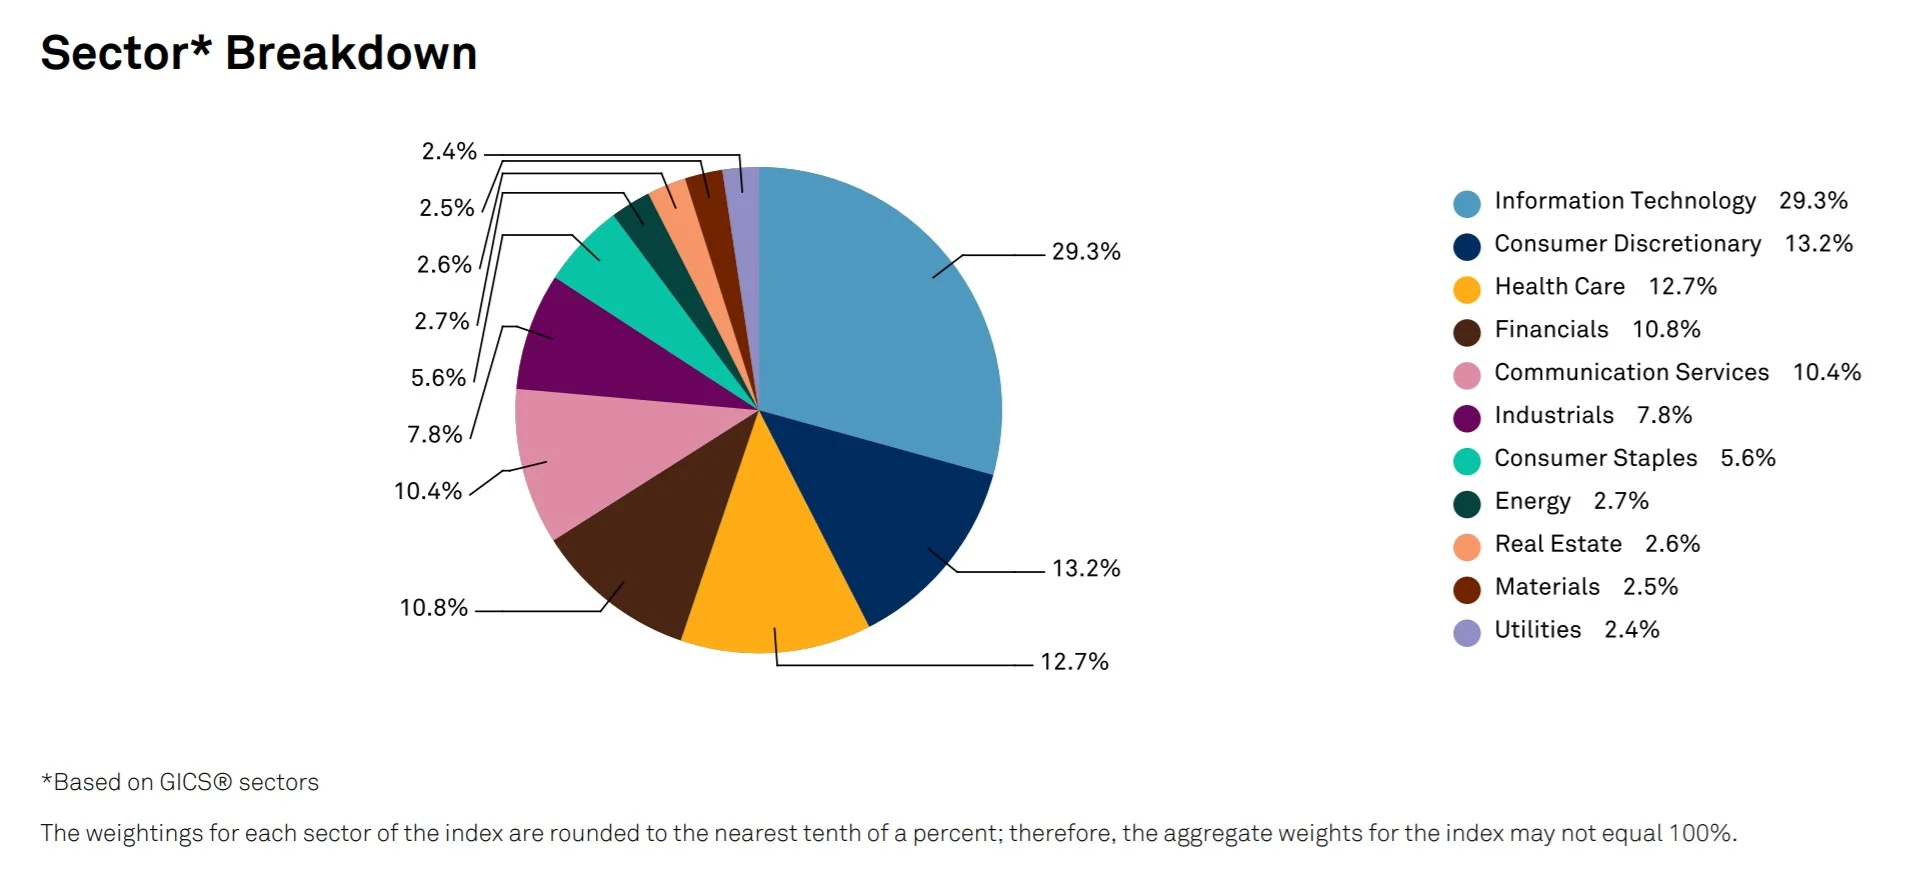
\includegraphics[width=0.6\textwidth]{figures/Sector-SP.png}
    \caption{S\&P 500 Sector Weightings}
    \label{fig:sector_sp}
\end{figure}

\paragraph{Stock Market Sectors}
The rationale behind this selection is multi-staged. Firstly, by including stocks from these predominant sectors, the portfolio captures the performance dynamics of the key drivers of the U.S. equity market. This approach ensures that the portfolio is both diversified and representative of broader market movements. Diversification across different sectors helps mitigate unsystematic risk associated with individual industries or companies, allowing the portfolio to benefit from growth opportunities while reducing the impact of sector-specific downturns.

Secondly, focusing on sectors that contribute most significantly to the S\&P 500 enhances the relevance of the study's findings to investors who benchmark their performance against this widely recognized index. The Information Technology sector, for example, encompasses leading companies in innovation and technology, significantly influencing market trends. The Health Care sector includes firms pivotal in advancing medical technology and pharmaceuticals, demonstrating resilience in various economic conditions.

Industrials and Consumer Discretionary sectors represent core components of the economy, reflecting business cycles and consumer spending patterns, respectively. The Financials sector plays a critical role in economic infrastructure, encompassing banking, insurance, and investment services. By selecting assets from these sectors, the portfolio encompasses areas crucial to economic growth and market capitalization.

This strategic selection aligns with the study's objective of developing a predictive portfolio optimization framework applicable to a realistic and impactful set of assets. It allows for testing the effectiveness of the proposed models and strategies in a context that is meaningful to investors and relevant to overall market performance. Moreover, by focusing on sectors that significantly influence the S\&P 500, the study ensures that its results have practical implications for portfolio management and investment decision-making.

\paragraph{Entropy Methods for Time Series Analysis}
To assess the complexity of the time-series data for these assets, we utilized entropy-based methods. Specifically, we employed the \texttt{OrdianlEntropy} package in Python, which provides time-efficient, ordinal pattern-based entropy algorithms for computing the complexity of one-dimensional time-series. This analysis informed our feature engineering process by highlighting the inherent unpredictability and dynamic behavior of the asset prices.

\subparagraph{Permutation Entropy (PE)}
Permutation Entropy (PE), introduced by Bandt and Pompe in 2002, is a measure of complexity that quantifies the diversity of ordinal patterns in a time series. It is based on the relative ordering of the values within embedding vectors derived from the time series.
Given a time series ${ x_t }_{t=1}^N$, the calculation of PE involves the following steps:

\begin{enumerate} \item \textbf{Embedding the Time Series:}
Choose an embedding dimension $m$ and time delay $\tau$, and construct embedding vectors:
\begin{equation}
    s_i = \left( x_i, x_{i+\tau}, x_{i+2\tau}, \dots, x_{i+(m-1)\tau} \right), \quad i = 1,2,\dots, N - (m -1)\tau.
\end{equation}

\item \textbf{Forming Ordinal Patterns:}

For each embedding vector $s_i$, determine the permutation $\pi_i$ that sorts its components in ascending order:
\begin{equation}
    s_i \rightarrow \left( x_{i+\tau(k_0)} \leq x_{i+\tau(k_1)} \leq \dots \leq x_{i+\tau(k_{m-1})} \right),
\end{equation}
where $(k_0, k_1, \dots, k_{m-1})$ represents the indices of the sorted components.

\item \textbf{Calculating Probabilities:}

Count the frequency of each of the $m!$ possible ordinal patterns $\pi_j$, and estimate their probabilities:
\begin{equation}
    p(\pi_j) = \frac{\text{Number of times pattern } \pi_j \text{ occurs}}{N - (m -1)\tau}.
\end{equation}

\item \textbf{Calculating Permutation Entropy:}

Compute the permutation entropy using Shannon's entropy formula:
\begin{equation}
    \mathrm{PE} = - \sum_{j=1}^{m!} p(\pi_j) \ln p(\pi_j).
\end{equation}

Normalize \ac{PE} by dividing by $\ln(m!)$ to ensure it ranges between 0 and 1:
\begin{equation}
    \mathrm{PE}_{\text{norm}} = \frac{\mathrm{PE}}{\ln(m!)}.
\end{equation}
\end{enumerate}

\begin{itemize} \item A \textbf{low PE} value indicates that the time series has a predictable or regular structure, with fewer unique ordinal patterns. \item A \textbf{high PE} value suggests that the time series is more complex or random, exhibiting a higher diversity of ordinal patterns. \end{itemize}


\subparagraph{Weighted Permutation Entropy (WPE)}
Weighted Permutation Entropy (WPE) enhances PE by incorporating the amplitude information of the time series. It assigns weights to ordinal patterns based on the values within the embedding vectors, thus accounting for both the order and magnitude of the data.
The calculation of \ac{WPE} involves the following steps:

\begin{enumerate} \item \textbf{Embedding and Ordinal Patterns:}
Follow steps 1 and 2 as in the calculation of PE to obtain the embedding vectors and their corresponding ordinal patterns.

\item \textbf{Assigning Weights:}

For each embedding vector $s_i$, calculate a weight $w_i$ based on the amplitude of its components. A common choice is the variance or absolute differences:
\begin{equation}
    w_i = \operatorname{Var}(s_i) = \frac{1}{m} \sum_{k=0}^{m-1} \left( x_{i+\tau k} - \bar{x}_i \right)^2,
\end{equation}
where $\bar{x}_i$ is the mean of the components of $s_i$.

\item \textbf{Calculating Weighted Probabilities:}

For each ordinal pattern $\pi_j$, compute the weighted probability:
\begin{equation}
    p_w(\pi_j) = \frac{\sum_{s_i \in \pi_j} w_i}{\sum_{i=1}^{N - (m -1)\tau} w_i}.
\end{equation}

\item \textbf{Calculating Weighted Permutation Entropy:}

Compute \ac{WPE} using the weighted probabilities:
\begin{equation}
    \mathrm{WPE} = - \sum_{j=1}^{m!} p_w(\pi_j) \ln p_w(\pi_j).
\end{equation}

Normalize WPE similarly to PE:
\begin{equation}
    \mathrm{WPE}_{\text{norm}} = \frac{\mathrm{WPE}}{\ln(m!)}.
\end{equation}
\end{enumerate}
\begin{itemize} \item \textbf{WPE} reflects both the diversity of ordinal patterns and the magnitude of fluctuations in the time series. \item It is more sensitive to significant changes in amplitude, making it useful for detecting volatility and abrupt transitions. \end{itemize}

\subparagraph{Dispersion Entropy (DE)}
Dispersion Entropy (DE), introduced by Rostaghi and Azami in 2016, is an entropy measure that accounts for both the ordering and dispersion of data by mapping the time series into a sequence of classes or symbols.
To calculate DE, follow these steps:

\begin{enumerate} \item \textbf{Mapping Data to Classes:}
Define $c$ classes and map each data point $x_t$ to a class label $k_t$ using a mapping function, such as:
\begin{equation}
    k_t = \left\lfloor c \cdot \frac{x_t - x_{\min} + \epsilon}{x_{\max} - x_{\min} + 2\epsilon} \right\rfloor + 1, \quad k_t \in \{1, 2, \dots, c\},
\end{equation}
where $x_{\min}$ and $x_{\max}$ are the minimum and maximum values of the time series, and $\epsilon$ is a small constant to prevent division by zero.

\item \textbf{Embedding:}

Form embedding vectors of class labels:
\begin{equation}
    s_i = \left( k_i, k_{i+\tau}, k_{i+2\tau}, \dots, k_{i+(m-1)\tau} \right).
\end{equation}

\item \textbf{Creating Dispersion Patterns:}

Each embedding vector $s_i$ represents a dispersion pattern $d_j$, where $j$ indexes the possible patterns.

\item \textbf{Calculating Probabilities:}

Count the frequency of each possible dispersion pattern and estimate their probabilities:
\begin{equation}
    p(d_j) = \frac{\text{Number of times pattern } d_j \text{ occurs}}{N - (m -1)\tau}.
\end{equation}

\item \textbf{Calculating Dispersion Entropy:}

Compute DE using:
\begin{equation}
    \mathrm{DE} = - \sum_{j=1}^{c^m} p(d_j) \ln p(d_j).
\end{equation}

Normalize DE by dividing by $\ln(c^m)$:
\begin{equation}
    \mathrm{DE}_{\text{norm}} = \frac{\mathrm{DE}}{\ln(c^m)}.
\end{equation}
\end{enumerate}

\begin{itemize} \item \textbf{DE} considers both the frequency and dispersion of data, providing a robust measure of complexity for non-stationary time series. \item It effectively captures changes in amplitude and is less sensitive to noise and outliers. \end{itemize}

\subparagraph{Choosing WPE and DE for Stock Price Analysis}
Analyzing stock prices requires accounting for both the order and magnitude of price changes due to the following reasons:

\subparagraph{Advantages of WPE}

Weighted Permutation Entropy (WPE) offers distinct benefits in the analysis of financial time series by effectively incorporating the amplitude of price changes into its computation. By weighting ordinal patterns, WPE not only captures the direction of changes but also accounts for their magnitude, making it particularly adept at identifying periods of heightened market volatility. This sensitivity to volatility is crucial for risk management, as it allows analysts to detect significant shifts in market behavior that could impact investment decisions. Furthermore, WPE strikes a balance between computational efficiency and analytical depth. It provides detailed insights into the complexity of financial data without requiring excessive computational resources, making it a practical tool for real-time and large-scale applications.


\subparagraph{Advantages of DE}

Dispersion Entropy (DE) excels in handling the complexities of non-stationary financial time series, which often exhibit trends, abrupt changes, and varying volatility. By mapping data into discrete classes, DE adapts effectively to non-stationarity, ensuring robust analysis across different market conditions. Its design also makes it less sensitive to noise and outliers, a significant advantage in the inherently noisy financial domain, where anomalies can skew traditional measures. DE provides a comprehensive view of market dynamics by considering both the frequency and amplitude of patterns, capturing subtle shifts in market behavior.

Another notable advantage of DE is its amplitude sensitivity. In financial markets, the size of price movements has a direct impact on returns and risks, and methods like DE that incorporate this information provide a richer understanding of market dynamics. Additionally, DE is particularly effective at detecting varying levels of volatility, which play a critical role in shaping investment strategies. Its ability to seamlessly handle the non-stationarity of stock prices, which often undergo regime changes and unpredictable trends, further solidifies its value in financial analysis.

Both WPE and DE offer robust tools for analyzing financial markets, with WPE emphasizing computational balance and volatility capture, while DE focuses on non-stationarity adaptation and comprehensive market understanding. Together, they provide complementary approaches to understanding the complexity of financial time series.
\subparagraph{Conclusion}
Weighted Permutation Entropy (WPE) and Dispersion Entropy (DE) prove to be superior tools compared to traditional Permutation Entropy when analyzing stock prices. These methods capture essential information about both the direction and magnitude of price movements, offering a more nuanced understanding of financial time-series data. Their ability to handle the inherent non-stationarity and volatility of financial markets makes them particularly well-suited for detecting patterns and trends that are often overlooked by simpler measures. Furthermore, WPE and DE provide more informative and sensitive complexity measures, enabling analysts to enhance asset selection and refine risk assessment strategies.

By utilizing \ac{WPE} and \ac{DE}, analysts and investors can achieve a deeper understanding of market behavior, uncovering the complexity and predictability of stock prices. These insights facilitate more informed decisions in selecting assets across different sectors, ultimately improving portfolio management and investment outcomes.
\subsection{Data Sources and Time Period}


To acquire the historical market data necessary for this study, we employed the EOD Historical Data API, a reputable and comprehensive source for end-of-day and historical financial data across various asset classes. The data retrieval process was automated using a Python script that constructs API requests based on the asset ticker, desired data period (e.g., daily, weekly), and specified date range.

For U.S.-listed assets, the script utilizes the endpoint format:

\begin{verbatim}
https://eodhd.com/api/eod/{ticker}.US?period={period}&api_token={api_token}
\end{verbatim}

where \texttt{\{ticker\}} represents the stock symbol, \texttt{\{period\}} denotes the data frequency, \texttt{\{api\_token\}} is the authentication token, and \texttt{\{start\_date\}} and \texttt{\{end\_date\}} define the data range. For Bitcoin (BTC), which is categorized differently in the API, the script accesses data using the endpoint:

\begin{verbatim}
https://eodhd.com/api/eod/BTC-USD.CC?period={period}&api_token={api_token}
\end{verbatim}

An API token, securely stored using environment variables to maintain confidentiality, is included in the requests for authentication. The script handles HTTP responses by checking for successful status codes and raising exceptions in case of errors, ensuring robust data retrieval.

Upon receiving a valid response, the JSON data is parsed into a pandas DataFrame for efficient data manipulation and analysis. The DataFrame includes essential financial indicators such as open, high, low, close prices, and trading volumes. The data is then saved as a CSV file in a structured directory hierarchy corresponding to each asset, following the path:

\begin{verbatim}
../Stocks/{ticker}/{ticker}_us_{period}.csv
\end{verbatim}

By automating the data fetching and saving process, we ensured consistency and repeatability in data collection of the whole pipeline. 
This method allowed us to systematically gather historical market data for all selected assets over the specified time periods, providing a reliable dataset for training the Gaussian Process Regression models and conducting backtesting for the portfolio optimization strategies. 
The use of the EOD Historical Data API ensured that the data was up-to-date and accurate, reflecting real market conditions essential for the validity of our analysis.
Also, for future work, the script can be easily adapted to retrieve data for additional assets or extend the time period, enabling further research and analysis in the financial domain.

\subsection{Data Preprocessing and Log Returns}
Data preprocessing and feature engineering are critical steps in preparing the dataset for modeling. They ensure that the data fed into the Gaussian Process Regression models are clean, consistent, and informative.

\paragraph{Use of Log Returns}

In this project, log returns are utilized for modeling asset price movements due to several compelling reasons that align with both theoretical and practical considerations in financial analysis.

\subparagraph{Theoretical Foundation in Finance}

Log returns are integral to many foundational financial models, such as the Black-Scholes option pricing model, which assume that asset prices follow a log-normal distribution. By using log returns, we align our modeling approach with these theoretical frameworks, facilitating more accurate and consistent analyses. \ac{GPR} models assume normally distributed outputs, and since log returns of log-normally distributed prices are normally distributed, this compatibility enhances the effectiveness of our predictive modeling.

\subparagraph{Stability Over Time}

Log returns exhibit greater stability compared to simple arithmetic returns, particularly in the presence of extreme outliers or during periods of high market volatility. They tend to smooth out spikes and reduce the impact of short-term noise, making the models less sensitive to sudden market anomalies. This stability is crucial for developing robust predictive models that can perform reliably under various market conditions.

\subparagraph{Time Consistency (Additivity)}

One of the key mathematical properties of log returns is their additive nature over time. The total log return over a period is the sum of the log returns over sub-periods:

\begin{equation}
\log\left( \frac{S_t}{S_0} \right) = \log\left( \frac{S_t}{S_{t-1}} \right) + \log\left( \frac{S_{t-1}}{S_{t-2}} \right) + \dots + \log\left( \frac{S_1}{S_0} \right),
\end{equation}

where $S_t$ is the asset price at time $t$. This additive property simplifies the computation of returns over arbitrary time horizons, such as weekly or monthly periods, by allowing us to sum daily log returns. It is particularly beneficial for forecasting and portfolio optimization over multi-day horizons, as it facilitates the aggregation of returns without the need for complex compounding calculations.

\subparagraph{Normalization of Price Scale}

Log returns are scale-invariant, meaning they standardize returns across assets regardless of their price levels. Whether an asset is priced at \$1 or \$1,000, the log return brings their percentage changes onto a consistent scale. This normalization simplifies comparisons across assets with vastly different price levels and reduces the need for additional data scaling or normalization procedures. It ensures that no single asset disproportionately influences the model due to its absolute price, allowing for a more balanced and equitable analysis within the portfolio.

\subparagraph{Conclusion}

By incorporating log returns into our modeling framework, we leverage their theoretical compatibility with financial models, enhance stability against market volatility, benefit from their time-additive properties, and achieve scale normalization across diverse assets. These advantages contribute to the robustness and accuracy of our Gaussian Process Regression models and improve the effectiveness of our dynamic portfolio optimization strategies.



\paragraph{Data Normalization and Scaling}

To bring all features onto a similar scale and improve the numerical stability of the models, we applied data normalization techniques. Specifically, we used min-max scaling to normalize the historical return features and the time index:

\begin{equation}
    X_{\text{normalized}} = \frac{X - X_{\text{min}}}{X_{\text{max}} - X_{\text{min}}},
\end{equation}

where $X$ represents the original feature values, and $X_{\text{min}}$ and $X_{\text{max}}$ are the minimum and maximum values of the feature, respectively. This scaling transforms the data to a [0, 1] range, facilitating efficient model training.

\paragraph{Treatment of Missing Data and Outliers}

Financial time-series data often contain missing values and outliers due to market closures, data recording errors, or extreme market events. To address missing data, we employed interpolation methods appropriate for time-series, such as linear interpolation and forward/backward filling, ensuring temporal continuity in the data.

Outliers were identified using the Interquartile Range (IQR) method:

\begin{equation}
    \text{IQR} = Q_3 - Q_1,
\end{equation}

where $Q_1$ and $Q_3$ are the first and third quartiles, respectively. Data points lying outside 1.5 times the IQR from the quartiles were considered outliers. We assessed these outliers to determine whether they were due to data errors or genuine market anomalies. Genuine outliers representing significant market movements were retained to preserve the dataset's integrity, while erroneous data points were corrected or removed.

\paragraph{Handling Missing Data with GPR}
\ac{GPR} is particularly effective in addressing missing data and managing outliers due to its probabilistic framework and ability to model uncertainties. As demonstrated in the figure, GPR leverages the observed data points to predict missing values by constructing a distribution over possible functions that fit the data. 
As shown in \ref{fig:gpr_missing_outliers} for each prediction, GPR provides both a mean estimate and a confidence interval that quantifies the uncertainty of the prediction. This feature allows it to interpolate missing data seamlessly while considering the underlying patterns and relationships in the time-series.

\begin{figure}[htbp]
    \centering
    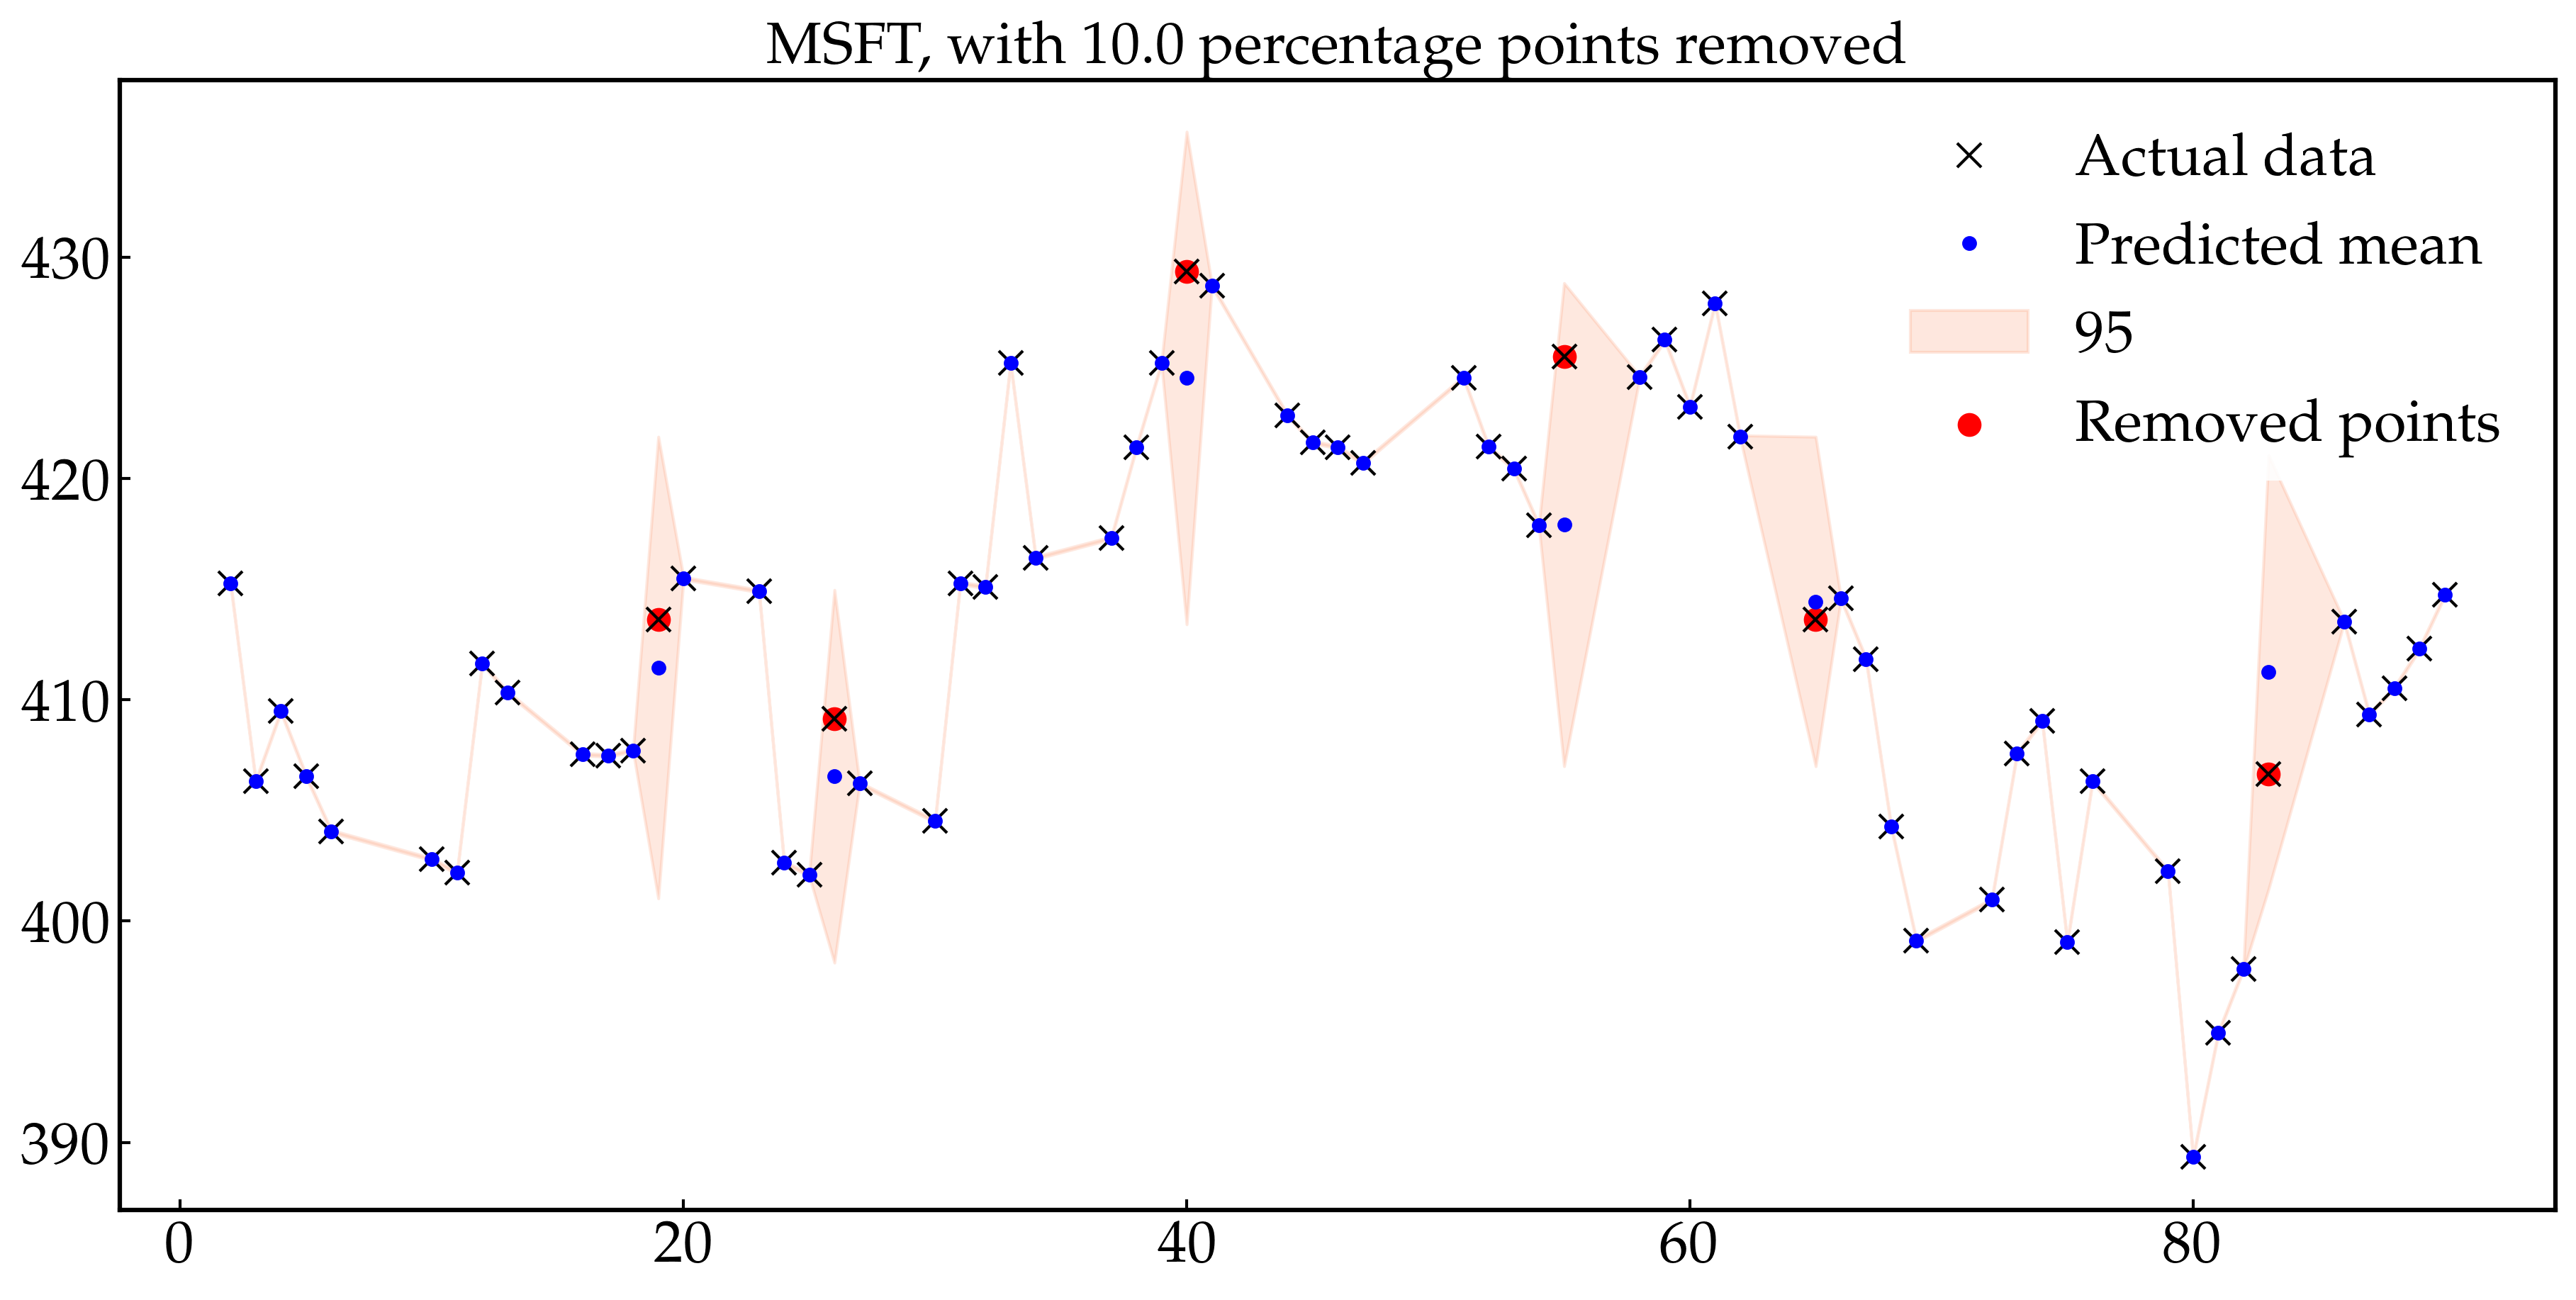
\includegraphics[width=0.6\textwidth]{figures/predicted_MSFT_with_removed.png}
    \caption{GPR Prediction with Missing Data and Outliers}
    \label{fig:gpr_missing_outliers}
\end{figure}

Furthermore, GPR handles outliers by naturally weighting data points according to their fit within the modeled distribution. Outliers, which deviate significantly from the predicted mean and exhibit higher uncertainty, are less influential in the model's predictions. This property prevents extreme values from distorting the regression output, making GPR robust in noisy and incomplete datasets. The ability to quantify uncertainty not only aids in filling missing data but also provides a valuable tool for identifying potential anomalies in the dataset, as seen in the highlighted regions of the plot. By incorporating these capabilities, GPR ensures that the dataset remains coherent and usable for subsequent analysis, such as predictive modeling and portfolio optimization.


\paragraph{Data Splitting and Cross-Validation}

The dataset was divided into training and testing sets to evaluate the model's predictive performance. The training set consisted of the first 80\% of the time period, while the remaining 20\% was reserved for testing. This chronological split respects the temporal order of the data, avoiding look-ahead bias.

To further validate the models, we used time-series cross-validation with a rolling window approach. In each iteration, the model was trained on a window of consecutive data points and tested on the subsequent period. This method provides a more robust assessment of the model's performance over time and simulates real-world forecasting conditions.

\paragraph{Sliding Window Approach}

To denoise the time-series data and reduce short-term fluctuations, we employed a sliding window approach using a centered rolling window mechanism. For each data point in the series, a window of a specified size $w$ was centered around it, and a statistical function was applied to the data within this window to compute a denoised value. The primary function used was the mean, though other functions could be applied as needed.

Formally, let $\{ x_t \}_{t=1}^T$ represent the original time-series data, and $\{ \tilde{x}_t \}_{t=1}^T$ denote the denoised series. The denoised value at time $t$, $\tilde{x}_t$, is calculated as:

\begin{equation}
\tilde{x}_t = \frac{1}{n_t} \sum_{i = t - k}^{t + k} x_i,
\end{equation}

where $k = \left\lfloor \frac{w}{2} \right\rfloor$, and $n_t$ is the number of data points within the window centered at time $t$. The window size $w$ is an odd integer to ensure symmetry around the central point. At the edges of the time-series (when $t - k < 1$ or $t + k > T$), the window is adjusted by including available data points, and the minimum number of periods is set to 1 to allow computation even with incomplete windows.

To handle any missing values that may arise at the edges due to insufficient data points, we applied forward and backward filling methods. Forward filling propagates the last observed non-missing value forward to fill subsequent missing positions, while backward filling fills missing values by propagating the next observed non-missing value backward. These steps ensure that the denoised series is complete and free from missing values.

This sliding window denoising process effectively smooths the data by averaging over the local neighborhood of each data point, reducing random noise while preserving significant trends and patterns. By enhancing the signal-to-noise ratio in the time-series, this approach improves the quality of the input data for the Gaussian Process Regression models, leading to better predictive performance and more reliable portfolio optimization decisions.

\paragraph{Gaussian Filter Denoising Method}

To further enhance the quality of the time-series data and reduce high-frequency noise, we employed the Gaussian filter denoising method. The Gaussian filter is a convolutional filter that applies a Gaussian kernel to smooth data by averaging neighboring points with weights determined by the Gaussian function. This technique preserves significant trends and patterns while effectively attenuating random fluctuations and noise.

The Gaussian kernel is defined by the Gaussian (normal) distribution function:

\begin{equation}
G(i) = \frac{1}{\sqrt{2\pi} \sigma} \exp\left( -\frac{i^2}{2\sigma^2} \right),
\end{equation}

where $i$ is the index distance from the central data point, and $\sigma$ is the standard deviation of the Gaussian distribution, controlling the degree of smoothing. A larger $\sigma$ results in a wider kernel and more extensive smoothing.

The denoised value at time $t$, $\tilde{x}_t$, is computed by convolving the original time-series data $x_t$ with the Gaussian kernel:

\begin{equation}
\tilde{x}_t = \sum_{i = -k}^{k} G(i) \cdot x_{t + i},
\end{equation}

where $k$ is the window size parameter determining the range of data points considered around time $t$.

In our implementation, we applied the Gaussian filter to the closing prices of the assets using a standard deviation $\sigma = 1$, which provides a balanced smoothing effect without overly distorting the data. The following code snippet illustrates the application of the Gaussian filter using the \texttt{gaussian\_filter} function from the SciPy library in Python:

\begin{lstlisting}[language=Python]
if isFiltered:
    df['filtered_close'] = gaussian_filter(df['close'], sigma=1)
\end{lstlisting}

In this code, \texttt{df['close']} represents the original closing price data, and \texttt{df['filtered\_close']} stores the denoised data after applying the Gaussian filter. The \texttt{isFiltered} flag allows for conditional application of the filtering process.

By using the Gaussian filter denoising method, we effectively reduced the impact of noise and short-term fluctuations in the financial time-series data. This preprocessing step enhances the signal-to-noise ratio, allowing the Gaussian Process Regression models to focus on underlying market trends and improving the accuracy of the return predictions. The combination of the sliding window approach and Gaussian filtering provides a robust methodology for data smoothing, contributing significantly to the reliability and performance of the predictive modeling and subsequent portfolio optimization.

The filtered data retained essential market movements while reducing random fluctuations, allowing the Gaussian Process Regression models to focus on meaningful signals.


\subsection{Summary}

By carefully selecting assets, sourcing reliable data, and meticulously preprocessing the dataset, we established a solid foundation for our predictive modeling. The combination of normalization, outlier treatment, strategic data splitting, and denoising ensured that the inputs to our models were of high quality. These steps are crucial for enhancing the performance of the Gaussian Process Regression models and, ultimately, for developing effective portfolio optimization strategies.



\section{Model Development}
In this section, we outline the development of the predictive framework and evaluation methodology for forecasting asset returns and optimizing portfolio allocations, namely trading strategies. The focus is on the performance metrics used to assess model effectiveness, as well as the selection of a baseline model for comparison with the Gaussian Process Regression (GPR) approach.

\subsection{Baseline Models}

To establish a reference point for the performance of the Gaussian Process Regression model, we selected the ARIMA (AutoRegressive Integrated Moving Average) model as the baseline.

\subsubsection{\ac{ARIMA} Model}

The \ac{ARIMA} model is a widely used time-series forecasting technique that combines autoregressive (AR), differencing (I), and moving average (MA) components. It is defined by three parameters: $p$, $d$, and $q$, where:

\begin{itemize}
    \item $p$ is the order of the autoregressive term.
    \item $d$ is the degree of differencing required to achieve stationarity.
    \item $q$ is the order of the moving average term.
\end{itemize}

The \ac{ARIMA} model forecasts the value at time $t$ as:

\begin{equation}
y_t = \phi_1 y_{t-1} + \phi_2 y_{t-2} + \dots + \phi_p y_{t-p} + \epsilon_t + \theta_1 \epsilon_{t-1} + \dots + \theta_q \epsilon_{t-q},
\end{equation}

where $\phi_i$ are the AR coefficients, $\theta_i$ are the MA coefficients, and $\epsilon_t$ is the white noise term.

\subsubsection{Rationale for Baseline Selection}

The \ac{ARIMA} model serves as an appropriate baseline because it is a well-established method for modeling time-series data and capturing trends and seasonality. While it is linear in nature, ARIMA provides a benchmark for assessing the added value of GPR, which can capture complex non-linear relationships and quantify uncertainty in predictions.

\subsection{Comparative Evaluation}

The performance of the \ac{GPR} model is compared against the \ac{ARIMA} baseline using the \ac{MSE} for predictive accuracy and the Sharpe Ratio for portfolio optimization outcomes. This dual evaluation approach ensures that the models are assessed comprehensively, both in terms of their forecasting ability and their impact on investment decisions. By demonstrating improvements over the \ac{ARIMA} model, the study highlights the effectiveness of \ac{GPR} in dynamic portfolio management.

\subsection{Performance Metrics}

To evaluate the performance of the predictive models and portfolio strategies, we employ the following metrics:

\subsubsection{Mean Squared Error (MSE)}

The Mean Squared Error (MSE) measures the accuracy of the model's predictions compared to the actual observed values. It is calculated as:

\begin{equation}
\text{MSE} = \frac{1}{n} \sum_{i=1}^{n} \left( y_i - \hat{y}_i \right)^2,
\end{equation}

where $y_i$ represents the actual value, $\hat{y}_i$ is the predicted value, and $n$ is the total number of predictions. A lower MSE indicates better predictive accuracy. This metric is particularly useful for evaluating the performance of GPR and baseline models in forecasting asset returns.

\subsubsection{Sharpe Ratio}

The Sharpe Ratio assesses the risk-adjusted performance of a portfolio, measuring the excess return per unit of risk. It is defined as:

\begin{equation}
\text{Sharpe Ratio} = \frac{E[R_p] - R_f}{\sigma_p},
\end{equation}

where $E[R_p]$ is the expected portfolio return, $R_f$ is the risk-free rate, and $\sigma_p$ is the portfolio's standard deviation of returns. A higher Sharpe Ratio indicates a more favorable trade-off between risk and return, making it a crucial metric for evaluating the effectiveness of the portfolio optimization strategies derived from the predicted returns.

\subsection{Multi-Input Gaussian Process Regression Model}

In this study, we developed a multi-input Gaussian Process Regression (GPR) model that incorporates multiple economic factors and time as input dimensions to predict the returns of individual stocks. The model combines features from a diverse set of assets and economic indicators, including Brent Oil prices, the US Dollar Index (DXY), the S\&P 500 Index, the Nasdaq 100 Index, Bitcoin (BTC), and gold prices (XAU/USD). This multi-input framework allows the model to capture intricate relationships between the target stock and broader market dynamics, enhancing its predictive power.

\subsubsection{Input Data and Feature Selection}

The input features for the GPR model were selected based on their correlation with the target stock. For each feature, we calculated the correlation between the feature's historical returns and the target stock's returns. Only features with an absolute correlation exceeding a predefined threshold were included in the model to ensure relevance and reduce noise in the predictions. This approach prioritizes the most influential economic factors while discarding irrelevant or weakly correlated inputs.

The final input matrix was constructed by concatenating the selected features along with time as an additional dimension. By including time, the model accounts for temporal trends and seasonality in the data, further improving its predictive capabilities.

\subsubsection{Composite Kernel for Multi-Dimensional Inputs}

To effectively model the multi-dimensional input space, we employed a composite kernel approach that assigns separate kernels to different input dimensions. Specifically:

\begin{itemize}
    \item One kernel was applied to the economic factors, allowing the model to learn the specific relationships between the target stock and each factor. This kernel captures the varying scales and complexities of the economic data.
    \item Another kernel was applied to the time dimension, enabling the model to account for temporal dependencies and trends. 
\end{itemize}

The composite kernel combines these two components multiplicatively, ensuring that the model can flexibly adjust to different input dimensions and set appropriate length scales for each. This design allows the GPR model to capture the unique characteristics of each feature while modeling their joint effects on the target stock's returns.

\subsubsection{Training and Testing Framework}

The training and testing process involved splitting the data into separate periods. The training set included data from the beginning of the time series up to a specified date, while the testing set encompassed the subsequent period. This split ensured that the model was evaluated on unseen data, simulating real-world forecasting conditions.

To further enhance the model's robustness, the noise variance in the GPR model was either fixed to a small value or optimized as a trainable parameter. This dual approach ensured flexibility in handling data with varying noise levels while preventing overfitting.

\subsubsection{Prediction and Evaluation}

Once the model was trained, it was used to predict the returns of the target stock over the testing period. The predictive mean and variance were computed for each test point, providing both point estimates and uncertainty bounds. The model's performance was evaluated using the Mean Squared Error (MSE), calculated for both normalized and denormalized data, to assess its accuracy in both relative and absolute terms.

By leveraging multi-input GPR with composite kernels, this approach captures the interplay between diverse economic factors, time, and stock returns. The flexibility in kernel design and inclusion of multi-dimensional inputs ensures that the model is both robust and adaptive, providing accurate predictions for individual stock performance in dynamic market environments.

\subsection{Hyperparameter Tuning}

Effective hyperparameter tuning is crucial for optimizing the performance of \ac{GPR} models, as it directly impacts the model's ability to fit the data and generalize to unseen samples. In this study, two distinct approaches were implemented for training \ac{GPR} models, differing in how the likelihood variance (noise variance) was treated during the optimization process. This subsection describes the methodologies and their respective advantages.

\subsubsection{Fixed Likelihood Variance}

In the first approach, the likelihood variance was fixed to a predefined value ($\sigma^2 = 10^{-3}$) and excluded from the training process. By keeping the noise variance constant, the optimization focuses solely on tuning the parameters of the kernel function, ensuring that the model does not overfit to noise in the data. This approach is computationally efficient and is particularly useful when the level of noise in the data is well-understood or consistent across the dataset. The training process involved minimizing the model's negative log marginal likelihood using the Scipy optimizer provided by \texttt{gpflow}:

\begin{equation}
\text{Negative Log Marginal Likelihood (NLML)} = -\log p(\mathbf{y} | \mathbf{X}, \boldsymbol{\theta}),
\end{equation}

where $\boldsymbol{\theta}$ represents the trainable kernel parameters.

\subsubsection{Trainable Likelihood Variance}

In the second approach, the likelihood variance was set as a trainable parameter, allowing the model to adaptively learn the optimal noise level from the data. This method is advantageous when the data contains varying levels of noise or when the noise characteristics are not well-understood. To enhance the robustness of this approach, multiple starting values for the likelihood variance were used ($10^{-5}$, $10^{-3}$, $10^{-1}$, $1.0$), ensuring that the optimization process explored a diverse range of initial configurations. For each starting variance, the model was trained using the Scipy optimizer, and the final negative log marginal likelihood was evaluated.

\begin{itemize}
    \item The model with the lowest final loss was selected as the best-performing model.
    \item This approach balances the trade-off between model flexibility and the risk of overfitting by optimizing both the kernel parameters and the likelihood variance.
\end{itemize}

\subsubsection{Comparison of Approaches}

Both approaches were evaluated based on their ability to minimize the negative log marginal likelihood and the predictive performance on the test dataset. The fixed likelihood variance method provided computational simplicity and reduced the risk of overfitting in scenarios with stable noise levels. Conversely, the trainable likelihood variance approach demonstrated higher adaptability, allowing the model to account for varying noise levels and capture the data's inherent uncertainty more effectively.

\subsubsection{Best Model Selection}

The trainable likelihood variance approach, with multiple initializations, identified the model configuration that minimized the negative log marginal likelihood. This model provided a balance between accurately capturing the signal and accounting for noise, making it the preferred choice for the Gaussian Process Regression framework used in this study.


\section{Forecasting Approach}
Describe the iterative forecasting method and how predictions are updated daily.

\subsection{Iterative Retraining for Sequential Predictions}

In addition to batch training and prediction, we implemented an iterative retraining approach for the Gaussian Process Regression (GPR) model. This method reflects a real-world scenario where new market data becomes available daily, requiring the model to be updated frequently to make accurate short-term predictions. In this approach, the GPR model is retrained daily using all available data up to the current day, and predictions are made for the next day. This process is repeated iteratively for five consecutive days to generate predictions for a five-day horizon.

\subsubsection{Methodology}

The iterative retraining approach involves the following steps:

\begin{enumerate}
    \item \textbf{Daily Data Integration:} At the start of each iteration, the most recent daily market data is fetched and added to the training dataset. This includes the latest values of the target stock and selected economic factors.
    \item \textbf{Training with Updated Data:} The GPR model is retrained using the expanded dataset, incorporating all historical data up to the current day. Both fixed and trainable likelihood variance configurations are evaluated to ensure robust performance.
    \item \textbf{Prediction for the Next Day:} Using the retrained model, predictions are made for the target stock's return for the next day. The predictive mean and variance are recorded for each iteration.
    \item \textbf{Iterative Execution:} Steps 1 through 3 are repeated iteratively, with each new day’s data being integrated into the model, until predictions are generated for all five future days.
\end{enumerate}

\subsubsection{Advantages of Iterative Retraining}

The iterative retraining approach offers several advantages:

\begin{itemize}
    \item \textbf{Real-Time Adaptation:} By retraining the model daily, it continuously adapts to the latest market conditions, ensuring that predictions remain relevant and responsive to recent trends.
    \item \textbf{Enhanced Short-Term Accuracy:} The use of updated data allows the model to account for the most recent market dynamics, improving the accuracy of short-term forecasts.
    \item \textbf{Uncertainty Quantification:} With each iteration, the GPR model provides a predictive mean and variance for the next day, enabling the assessment of uncertainty in the predictions. This is particularly useful for risk-aware decision-making in portfolio management.
\end{itemize}

\subsubsection{Performance Evaluation}

To evaluate the effectiveness of this approach, the Mean Squared Error (MSE) was calculated for both normalized and denormalized predicted returns across the five days. The iterative predictions were also compared against actual returns to assess the model's ability to track short-term market movements. Additionally, the cumulative performance over the five-day horizon was analyzed to understand the overall impact of daily updates on predictive accuracy.

\subsubsection{Practical Application}

This iterative retraining approach closely mimics real-world trading scenarios where investors rely on daily market updates to make decisions. By retraining the model with the latest data and predicting only one day ahead, this method ensures that the predictions are both timely and aligned with current market conditions. This sequential prediction framework provides a robust foundation for dynamic portfolio management, enabling more accurate and adaptive asset allocation strategies.



\section{Portfolio Optimization Strategies}

\subsection{Traditional Strategies}
\subsubsection{Maximum Return Strategy Formulation}

The maximum return strategy aims to maximize the expected return of a portfolio while considering risk constraints and incorporating regularization penalties such as L1/L2 norms and transaction costs. The optimization problem is formulated based on the given code snippet and can be expressed mathematically as follows.

Let:

\begin{itemize}
    \item \( \mathbf{w} \in \mathbb{R}^n \) be the vector of portfolio weights for \( n \) assets.
    \item \( \boldsymbol{\mu} \in \mathbb{R}^n \) be the vector of expected returns for each asset.
    \item \( \Sigma \in \mathbb{R}^{n \times n} \) be the covariance matrix of asset returns.
    \item \( \sigma_{\text{max}} \) be the maximum allowable portfolio volatility.
    \item \( \mathcal{R}(\mathbf{w}) \) be the regularization penalty function, which may include L1/L2 penalties and transaction costs.
\end{itemize}

The optimization problem is:

\[
\begin{aligned}
\min_{\mathbf{w}} & \quad -\mathbf{w}^\top \boldsymbol{\mu} + \mathcal{R}(\mathbf{w}) \\
\text{subject to} & \quad \sqrt{\mathbf{w}^\top \Sigma \mathbf{w}} \leq \sigma_{\text{max}} \\
& \quad \sum_{i=1}^n w_i = 1 \\
& \quad w_i \geq 0, \quad \forall i \in \{1, \dots, n\}
\end{aligned}
\]

\paragraph{Objective Function}

The objective function consists of two components:

\begin{enumerate}
    \item \textbf{Negative Expected Return}: \( -\mathbf{w}^\top \boldsymbol{\mu} \)
    \item \textbf{Regularization Penalty}: \( \mathcal{R}(\mathbf{w}) \)
\end{enumerate}

By minimizing the negative expected return, we effectively maximize the portfolio's expected return. The regularization penalty \( \mathcal{R}(\mathbf{w}) \) accounts for additional considerations such as promoting sparsity (L1 regularization), preventing overfitting (L2 regularization), and minimizing transaction costs.

\paragraph{Constraints}

The constraints ensure that:

\begin{itemize}
    \item \textbf{Volatility Constraint}: The portfolio's volatility does not exceed \( \sigma_{\text{max}} \):

    \[
    \sqrt{\mathbf{w}^\top \Sigma \mathbf{w}} \leq \sigma_{\text{max}}
    \]

    \item \textbf{Full Investment Constraint}: The sum of the portfolio weights equals 1:

    \[
    \sum_{i=1}^n w_i = 1
    \]

    \item \textbf{No Short-Selling Constraint}: All portfolio weights are non-negative:

    \[
    w_i \geq 0, \quad \forall i
    \]
\end{itemize}

\paragraph{Regularization Penalty}

The regularization penalty \( \mathcal{R}(\mathbf{w}) \) can be detailed as:

\[
\mathcal{R}(\mathbf{w}) = \lambda_1 \|\mathbf{w}\|_1 + \lambda_2 \|\mathbf{w}\|_2^2 + \gamma \sum_{i=1}^n |w_i - w_i^{\text{prev}}|
\]

where:

\begin{itemize}
    \item \( \|\mathbf{w}\|_1 = \sum_{i=1}^n |w_i| \) is the L1 norm, promoting sparsity in the portfolio weights.
    \item \( \|\mathbf{w}\|_2^2 = \sum_{i=1}^n w_i^2 \) is the squared L2 norm, preventing extreme weight allocations.
    \item \( w_i^{\text{prev}} \) is the previous weight of asset \( i \), accounting for transaction costs when adjusting the portfolio.
    \item \( \lambda_1, \lambda_2, \gamma \geq 0 \) are hyperparameters controlling the influence of each penalty component.
\end{itemize}

\paragraph{Optimization Method}

The optimization problem is solved using the Sequential Least Squares Programming (SLSQP) algorithm, which is suitable for constrained nonlinear optimization. The method minimizes the objective function while satisfying the specified constraints.

\[
\text{Result} = \arg\min_{\mathbf{w}} \left( -\mathbf{w}^\top \boldsymbol{\mu} + \mathcal{R}(\mathbf{w}) \right)
\]

\[
\text{subject to constraints}
\]

\paragraph{Implementation Notes}

In our implementation:

\begin{itemize}
    \item The function \texttt{returns\_objective} computes the objective function.
    \item The \texttt{maximize\_returns} method sets up the optimization problem, including the volatility constraint and any additional constraints.
    \item Regularization and transaction costs are incorporated through the \texttt{total\_penalty} function.
\end{itemize}

By formulating the strategy in this manner, the model seeks the optimal balance between maximizing returns and controlling for risk and costs, resulting in a robust and practical portfolio optimization solution.


\subsubsection{Maximum Sharpe Ratio Optimization}

The maximum Sharpe ratio optimization aims to maximize the portfolio's Sharpe ratio, which is a measure of risk-adjusted return. This involves finding the optimal portfolio weights that maximize the expected return minus the risk-free rate, divided by the portfolio's volatility, while also incorporating regularization penalties such as L1/L2 norms and transaction costs.

Let:

\begin{itemize}
    \item \( \mathbf{w} \in \mathbb{R}^n \) be the vector of portfolio weights for \( n \) assets.
    \item \( \boldsymbol{\mu} \in \mathbb{R}^n \) be the vector of expected returns for each asset.
    \item \( \Sigma \in \mathbb{R}^{n \times n} \) be the covariance matrix of asset returns.
    \item \( r_f \) be the risk-free rate.
    \item \( \mathcal{R}(\mathbf{w}) \) be the regularization penalty function, which may include L1/L2 penalties and transaction costs.
\end{itemize}

The Sharpe ratio \( S(\mathbf{w}) \) is defined as:

\[
S(\mathbf{w}) = \frac{\mathbf{w}^\top \boldsymbol{\mu} - r_f}{\sqrt{\mathbf{w}^\top \Sigma \mathbf{w}}}
\]

The optimization problem is:

\[
\begin{aligned}
\max_{\mathbf{w}} & \quad S(\mathbf{w}) - \mathcal{R}(\mathbf{w}) \\
\text{subject to} & \quad \sum_{i=1}^n w_i = 1 \\
& \quad w_i \geq 0, \quad \forall i \in \{1, \dots, n\}
\end{aligned}
\]

Since optimization algorithms typically perform minimization, we can reformulate the problem as minimizing the negative Sharpe ratio plus the regularization penalty:

\[
\begin{aligned}
\min_{\mathbf{w}} & \quad -\frac{\mathbf{w}^\top \boldsymbol{\mu} - r_f}{\sqrt{\mathbf{w}^\top \Sigma \mathbf{w}}} + \mathcal{R}(\mathbf{w}) \\
\text{subject to} & \quad \sum_{i=1}^n w_i = 1 \\
& \quad w_i \geq 0, \quad \forall i
\end{aligned}
\]

\paragraph{Objective Function}

The objective function consists of:

\begin{enumerate}
    \item \textbf{Negative Sharpe Ratio}: \( -\dfrac{\mathbf{w}^\top \boldsymbol{\mu} - r_f}{\sqrt{\mathbf{w}^\top \Sigma \mathbf{w}}} \)
    \item \textbf{Regularization Penalty}: \( \mathcal{R}(\mathbf{w}) \)
\end{enumerate}

By minimizing the negative Sharpe ratio, we effectively maximize the Sharpe ratio, thus maximizing the portfolio's risk-adjusted return.

\paragraph{Constraints}

The constraints ensure that:

\begin{itemize}
    \item \textbf{Full Investment Constraint}: The sum of the portfolio weights equals 1:

    \[
    \sum_{i=1}^n w_i = 1
    \]

    \item \textbf{No Short-Selling Constraint}: All portfolio weights are non-negative:

    \[
    w_i \geq 0, \quad \forall i
    \]
\end{itemize}

\paragraph{Regularization Penalty}

The regularization penalty \( \mathcal{R}(\mathbf{w}) \) includes both L1/L2 penalties and transaction costs, and can be expressed as:

\[
\mathcal{R}(\mathbf{w}) = \lambda_1 \|\mathbf{w}\|_1 + \lambda_2 \|\mathbf{w}\|_2^2 + \gamma \sum_{i=1}^n |w_i - w_i^{\text{prev}}|
\]

where:

\begin{itemize}
    \item \( \|\mathbf{w}\|_1 = \sum_{i=1}^n |w_i| \) is the L1 norm, promoting sparsity in the portfolio weights.
    \item \( \|\mathbf{w}\|_2^2 = \sum_{i=1}^n w_i^2 \) is the squared L2 norm, preventing extreme weight allocations.
    \item \( w_i^{\text{prev}} \) is the previous weight of asset \( i \), accounting for transaction costs when adjusting the portfolio.
    \item \( \lambda_1, \lambda_2, \gamma \geq 0 \) are hyperparameters controlling the influence of each penalty component.
\end{itemize}

\paragraph{Optimization Method}

The optimization problem is solved using the Sequential Least Squares Programming (SLSQP) algorithm, which is suitable for constrained nonlinear optimization. The method minimizes the objective function while satisfying the specified constraints:

\[
\text{Result} = \arg\min_{\mathbf{w}} \left( -\dfrac{\mathbf{w}^\top \boldsymbol{\mu} - r_f}{\sqrt{\mathbf{w}^\top \Sigma \mathbf{w}}} + \mathcal{R}(\mathbf{w}) \right)
\]

\[
\text{subject to constraints}
\]

\paragraph{Implementation Notes}

In our implementation:

\begin{itemize}
    \item The function \texttt{objective} computes the negative Sharpe ratio plus regularization penalties.
    \item The \texttt{optimize\_portfolio} method sets up the optimization problem, including the necessary constraints.
    \item Regularization and transaction costs are incorporated through the \texttt{total\_penalty} function.
\end{itemize}

By formulating the strategy in this manner, the model seeks to maximize the portfolio's risk-adjusted return while controlling for risk and costs, resulting in an efficient and practical portfolio optimization solution.


\subsection{Dynamic Strategy}
In this project, we specifically designed a dynamic strategy, that is to decide at each time point which portfolio optimization strategy to use based on the predicted market conditions. The dynamic strategy involves two main components: the regime detection model and the strategy selection mechanism.
For the regime detection model, we employed a Probability Estimation Model and a Expected Value Comparison Method to identify distinct regimes based on the predicted returns and uncertainties. 

For the strategy selection mechanism, we developed a Decision Rule that determines the optimal portfolio optimization strategy based on the detected regime. The dynamic strategy aims to adapt to changing market conditions and optimize portfolio allocations accordingly, enhancing the robustness and performance of the investment approach.
\subsubsection{Probability Estimation: $P(S_1 > S_2)$}

When estimating the probability $P(S_1 > S_2)$ for two random variables $S_1$ and $S_2$, the methodology depends on the nature of their distributions and their dependence structure. This section outlines three approaches: numerical integration, Monte Carlo simulation, and the use of copulas for dependent variables.

\paragraph{Numerical Integration}

If the probability density functions (PDFs) of $S_1$ and $S_2$ are known, the probability $P(S_1 > S_2)$ can be expressed as:
\begin{equation}
P(S_1 > S_2) = \int_{-\infty}^\infty \int_{y}^\infty f_{S_1}(x) f_{S_2}(y) \, dx \, dy,
\end{equation}
where:
\begin{itemize}
    \item $f_{S_1}(x)$ is the PDF of $S_1$,
    \item $f_{S_2}(y)$ is the PDF of $S_2$.
\end{itemize}

This double integral represents the joint probability over the region where $S_1 > S_2$, and it requires numerical methods for evaluation when closed-form solutions are unavailable.


\paragraph{Copulas for Dependence}

Especially, When $S_1$ and $S_2$ are dependent, the joint distribution can be modeled using a copula. A copula is a function that describes the dependence structure between random variables, linking their marginal distributions. Let $F_{S_1}(x)$ and $F_{S_2}(y)$ represent the cumulative distribution functions (CDFs) of $S_1$ and $S_2$, respectively. The joint CDF can be expressed as:
\begin{equation}
F_{S_1, S_2}(x, y) = C(F_{S_1}(x), F_{S_2}(y)),
\end{equation}
where $C(u, v)$ is the copula function.

The probability $P(S_1 > S_2)$ can then be computed as:
\begin{equation}
P(S_1 > S_2) = \int_{-\infty}^\infty \int_{y}^\infty \frac{\partial^2 C(F_{S_1}(x), F_{S_2}(y))}{\partial u \partial v} \, dx \, dy.
\end{equation}

The steps to compute this are:
\begin{enumerate}
    \item Determine the marginal distributions $F_{S_1}(x)$ and $F_{S_2}(y)$ for $S_1$ and $S_2$.
    \item Select an appropriate copula function $C(u, v)$ based on the dependence structure (e.g., Gaussian, Clayton, or Gumbel copulas).
    \item Use numerical methods to evaluate the double integral above.
\end{enumerate}

Copulas are particularly effective when the marginal distributions are non-normal or when the dependence structure is non-linear and cannot be captured by simple correlation measures.

\paragraph{Monte Carlo Methods}

If the distributions of $S_1$ and $S_2$ are not explicitly known but sampling from these distributions is possible, a Monte Carlo simulation can be used to estimate $P(S_1 > S_2)$. The steps are as follows:
\begin{enumerate}
    \item Generate $N$ independent samples $S_1^{(i)}$ and $S_2^{(i)}$ from the respective distributions of $S_1$ and $S_2$.
    \item Count the number of instances where $S_1^{(i)} > S_2^{(i)}$. Denote this count by $n$.
    \item Estimate the probability as:
    \begin{equation}
    P(S_1 > S_2) \approx \frac{n}{N},
    \end{equation}
    where
    \begin{equation}
    n = \sum_{i=1}^N \mathbb{I}(S_1^{(i)} > S_2^{(i)}),
    \end{equation}
    and $\mathbb{I}(\cdot)$ is the indicator function, which equals 1 if the condition is true and 0 otherwise.
\end{enumerate}

Monte Carlo simulation is particularly useful for complex distributions or dependent variables, where analytical integration is impractical. In our case, we have multiple assets with potentially non-normal distributions and complex dependencies, making Monte Carlo methods a valuable tool for estimating $P(S_1 > S_2)$.
Specifically, we will use Monte Carlo simulation to estimate the probability of one asset outperforming another in our portfolio optimization strategies. And we chose a sample size of $N = 10,000$ to ensure accurate probability estimates.

\paragraph{Comparison of Methods}

\begin{itemize}
    \item \textbf{Numerical Integration:} Provides an exact solution given the PDFs of $S_1$ and $S_2$, but computationally intensive for high-dimensional problems or non-standard distributions.
    \item \textbf{Copulas:} Allows modeling of complex dependence structures, particularly useful for non-normal distributions or asymmetric dependencies.
    \item \textbf{Monte Carlo Simulation:} Flexible and practical alternative when sampling is straightforward, though its accuracy depends on the number of samples $N$.
\end{itemize}

Each method has its strengths and limitations, given the availability of distributional information and computational resources of our case, we chose to use Monte Carlo simulation for estimating $P(S_1 > S_2)$.


\paragraph{Strategy switching criteria}
Describe the criteria for switching between portfolio optimization strategies based on the estimated probability $P(S_1 > S_2)$.
We set a threshold probability $\tau$ such that if $P(S_1 > S_2) > \tau$, the strategy with the higher expected return is selected, and if $P(S_1 > S_2) \leq \tau$, the strategy with the lower volatility is chosen. This threshold ensures that the strategy selection is based on a balance between return and risk, incorporating the estimated probability of one asset outperforming the other.
\subsubsection{Expected Value Comparison}
The Expected Value Comparison method involves comparing the expected values of two time points distribution to determine the optimal choice. This approach is based on the principle of maximizing the expected return or Sharpe ratio while considering the estimated probabilities of each strategy's performance. The Expected Value Comparison method is particularly useful for dynamic portfolio optimization, where the selection of strategies is based on their expected outcomes under different market conditions.

The dynamic strategy employs a decision-making process based on the comparison of expected portfolio returns using previous and current predictions. The core idea is to adaptively switch between maximizing returns and minimizing volatility (uncertainty) depending on the anticipated changes in the market. The strategy aims to optimize the portfolio by considering not only the expected returns but also transaction costs associated with rebalancing.

Let:

\begin{itemize}
    \item \( \boldsymbol{\mu}_A \in \mathbb{R}^n \) be the vector of expected returns at time \( t-1 \).
    \item \( \boldsymbol{\mu}_B \in \mathbb{R}^n \) be the vector of expected returns at time \( t \).
    \item \( \mathbf{w}_{\text{prev}} \in \mathbb{R}^n \) be the portfolio weights optimized at time \( t-1 \).
    \item \( \lambda_{\text{tx}} \) be the transaction cost rate.
\end{itemize}

\paragraph{Decision Logic}

The strategy proceeds as follows and is updated at each time step, for each round the decision flow can be seen in the flowchart below:

\begin{enumerate}
    \item \textbf{Initialization}: For the first time step (\( t = 0 \)), where no previous weights exist, the strategy allocates weights by maximizing returns under a volatility constraint:

    \[
    \mathbf{w}_0 = \arg\min_{\mathbf{w}} \left( -\boldsymbol{\mu}_B^\top \mathbf{w} + \mathcal{R}(\mathbf{w}) \right)
    \]
    
    subject to the constraints specified in the maximum return strategy.

    \item \textbf{Expected Returns Calculation}: For \( t \geq 1 \), calculate the expected portfolio returns at times \( t-1 \) and \( t \) using the previous optimal weights \( \mathbf{w}_{\text{prev}} \):

    \[
    R_A = \boldsymbol{\mu}_A^\top \mathbf{w}_{\text{prev}}
    \]
    \[
    R_B = \boldsymbol{\mu}_B^\top \mathbf{w}_{\text{prev}}
    \]

    \item \textbf{Comparison of Expected Returns}:
    \begin{itemize}
        \item If \( R_A > R_B \) (the expected return is increasing), it suggests that the current allocation may yield higher returns in the next period, which indicates a favorable market condition. Therefore, the strategy opts to \textbf{maximize returns} by solving:

        \[
        \mathbf{w}_t = \arg\min_{\mathbf{w}} \left( -\boldsymbol{\mu}_B^\top \mathbf{w} + \mathcal{R}(\mathbf{w}) \right)
        \]
        
        subject to the constraints specified in the maximum return strategy.

        \item If \( R_A \leq R_B \) (the expected return is decreasing), we adopt a more conservative strategy to avoid potential market risks, which is to choose \textbf{minimize volatility} by solving:

        \[
        \mathbf{w}_t = \arg\min_{\mathbf{w}} \left( \sqrt{\mathbf{w}^\top \Sigma_B \mathbf{w}} + \mathcal{R}(\mathbf{w}) \right)
        \]
        
        subject to the constraints specified in the minimum volatility approach, where \( \Sigma_B \) is the covariance matrix at time \( t \).
    \end{itemize}

    \item \textbf{Transaction Cost Adjustment}: Compute the transaction costs incurred due to rebalancing:

    \[
    \text{TransactionCost} = \lambda_{\text{tx}} \sum_{i=1}^n |w_{i, t} - w_{i, t-1}|
    \]

    \item \textbf{Realized Return Calculation}: Calculate the realized change in expected return after accounting for transaction costs:

    \[
    \Delta R_{\text{realized}} = (R_B - R_A) - \text{TransactionCost}
    \]

    \item \textbf{Strategy Adjustment}:
    \begin{itemize}
        \item If \( \Delta R_{\text{realized}} > 0 \), the expected improvement in return outweighs the transaction costs, and the new weights \( \mathbf{w}_t \) are adopted.
        \item If \( \Delta R_{\text{realized}} \leq 0 \), the transaction costs negate the benefits of rebalancing, and the strategy \textbf{reverts to the previous weights}:

        \[
        \mathbf{w}_t = \mathbf{w}_{\text{prev}}
        \]
    \end{itemize}
\end{enumerate}

\begin{figure}[htbp]
\centering
\scalebox{0.8}{
\begin{tikzpicture}[scale=0.1, node distance=2.5cm, auto, >=latex']
    % Define block styles
    \tikzstyle{startstop} = [rectangle, rounded corners, minimum width=3cm, minimum height=1cm, text centered, draw=black, fill=gray!10]
    \tikzstyle{process} = [rectangle, minimum width=3cm, minimum height=1cm, text centered, draw=black, fill=blue!10]
    \tikzstyle{decision} = [diamond, aspect=2, text centered, draw=black, fill=green!10]
    \tikzstyle{arrow} = [thick,->,>=stealth]

    % Nodes
    \node [startstop] (start) {Start};
    \node [decision, below of=start, node distance=2.5cm, align=center] (prev_weights) {Previous Weights \\ Exist ?};
    \node [process, below of=prev_weights, node distance=3cm, align=center] (init_alloc) {Maximize Returns \\ Volatility Constraint};
    \node [process, right of=prev_weights, node distance=6cm, align=center] (calc_exp_returns) {Calculate Expected Returns \\ $R_A = \boldsymbol{\mu}_A^\top \mathbf{w}_{\text{prev}}$ \\ $R_B = \boldsymbol{\mu}_B^\top \mathbf{w}_{\text{prev}}$};
    \node [decision, below of=calc_exp_returns, node distance=3cm, align=center] (compare_returns) {$R_A < R_B$?};
    \node [process, right of=compare_returns, node distance=7.5cm, align=center] (max_returns) {Maximize Returns};
    \node [process, below of=compare_returns, node distance=3cm, align=center] (min_uncertainty) {Minimize Volatility};
    \node [process, below of=min_uncertainty, node distance=2cm, align=center] (compute_trx_costs) {Compute Transaction Costs \\ $\Delta R_{\text{realized}} = (R_B - R_A) - \text{TransactionCost}$};
    \node [decision, below of=compute_trx_costs, node distance=3cm, align=center] (delta_R_pos) {$\Delta R_{\text{realized}} > 0$?};
    \node [process, below of=delta_R_pos, node distance=3cm, align=center] (adopt_new_weights) {Adopt New Weights \\ $\mathbf{w}_t$};
    \node [process, right of=delta_R_pos, node distance=5cm, align=center] (keep_prev_weights) {Keep Previous Weights \\ $\mathbf{w}_t = \mathbf{w}_{\text{prev}}$};
    \node [startstop, below of=adopt_new_weights, node distance=2.5cm, align=center] (end) {End};

    % Paths
    \draw [arrow] (start) -- (prev_weights);
    \draw [arrow] (prev_weights) -- node[left] {No} (init_alloc);
    \draw [arrow] (prev_weights) -- node[above] {Yes} (calc_exp_returns);
    \draw [arrow] (init_alloc) |- (end);
    \draw [arrow] (calc_exp_returns) -- (compare_returns);
    \draw [arrow] (compare_returns) -- node[left] {No} (min_uncertainty);
    \draw [arrow] (compare_returns) -- node[above] {Yes} (max_returns);
    \draw [arrow] (max_returns) |- (end);
    \draw [arrow] (min_uncertainty) -- (compute_trx_costs);
    \draw [arrow] (compute_trx_costs) -- (delta_R_pos);
    \draw [arrow] (delta_R_pos) -- node[left] {Yes} (adopt_new_weights);
    \draw [arrow] (delta_R_pos) -- node[above] {No} (keep_prev_weights);
    \draw [arrow] (adopt_new_weights) -- (end);
    \draw [arrow] (keep_prev_weights) |- (end);
\end{tikzpicture}
}
\caption{Decision Flowchart for the Dynamic Strategy}
\end{figure}


\paragraph{Rationale}

The strategy's decision criteria are designed to balance the trade-off between expected returns and transaction costs:
By comparing \( R_A \) and \( R_B \), the strategy assesses whether the expected return is improving or deteriorating.
 Maximizing returns when the expected return is decreasing attempts to counteract the anticipated decline by seeking higher-return allocations.
 Minimizing volatility when the expected return is increasing adopts a conservative stance to preserve gains while benefiting from favorable market conditions.
Incorporating transaction costs ensures that rebalancing decisions are economically justified, preventing unnecessary trading that could erode returns.


\paragraph{Conclusion}

The dynamic strategy effectively combines elements of both the maximum return and minimum volatility strategies, switching between them based on expected changes in returns and considering transaction costs. By doing so, it aims to optimize the portfolio's performance in varying market conditions while maintaining a balance between risk and return.


\section{Backtesting Framework}

In this section, we describe the backtesting framework used to evaluate the performance of the portfolio optimization strategies. The backtesting process involves simulating the optimized portfolios over historical data to assess their effectiveness in real-world scenarios. The framework utilizes two primary classes, \texttt{Return} and \texttt{Volatility}, to calculate portfolio returns and volatilities, respectively.

\subsection{Overview of the Backtesting Process}

The backtesting process involves the following steps:

\begin{enumerate}
    \item \textbf{Data Preparation}: Historical asset returns and predicted volatilities are collected for the assets under consideration.
    \item \textbf{Portfolio Optimization}: The optimization strategies (e.g., maximum Sharpe ratio, maximum return, minimum volatility) are applied to generate optimal portfolio weights.
    \item \textbf{Return and Volatility Calculation}: The \texttt{Return} and \texttt{Volatility} classes compute the daily portfolio returns, cumulative returns, transaction costs, and portfolio volatilities.
    \item \textbf{Performance Evaluation}: Key performance metrics such as cumulative return, cumulative transaction costs, portfolio variance, and Sharpe ratio are calculated to evaluate the strategies.
\end{enumerate}

\subsection{Return Calculation}

\subsubsection{Return Class Implementation}

The \texttt{Return} class is designed to calculate portfolio returns based on asset returns and portfolio weights, accounting for transaction costs. It is initialized with:

\begin{itemize}
    \item \texttt{asset\_returns}: A NumPy array of asset returns.
    \item \texttt{weights}: A NumPy array of portfolio weights, where each row corresponds to a specific time period.
    \item \texttt{transaction\_cost\_rate}: A scalar representing the transaction cost rate (default is 0).
\end{itemize}

The class provides methods to calculate:

\begin{itemize}
    \item \textbf{Daily Portfolio Returns}: Computes the net portfolio returns for each day, considering transaction costs.
    \item \textbf{Cumulative Return}: Calculates the cumulative return of the portfolio over the backtesting period.
    \item \textbf{Cumulative Transaction Costs}: Sums up the transaction costs incurred over the backtesting period.
    \item \textbf{Daily Transaction Costs}: Provides the transaction costs for each day.
\end{itemize}

\paragraph{Daily Portfolio Return Calculation}

The daily portfolio return \( r_{\text{net}, t} \) on day \( t \) is calculated as:

\[
r_{\text{net}, t} = \mathbf{w}_t^\top \mathbf{r}_t - \text{Transaction Cost}_t
\]

where:

\begin{itemize}
    \item \( \mathbf{w}_t \) is the portfolio weight vector at time \( t \).
    \item \( \mathbf{r}_t \) is the asset return vector at time \( t \).
    \item \( \text{Transaction Cost}_t \) is the transaction cost incurred on day \( t \), calculated as:

    \[
    \text{Transaction Cost}_t = \lambda_{\text{tx}} \sum_{i=1}^n |w_{i, t} - w_{i, t-1}|
    \]

    with \( \lambda_{\text{tx}} \) being the transaction cost rate, and \( w_{i, t} \) being the weight of asset \( i \) at time \( t \).
\end{itemize}

\paragraph{Cumulative Return Calculation}

The cumulative return over \( T \) days is calculated as:

\[
\text{Cumulative Return} = \prod_{t=1}^T (1 + r_{\text{net}, t}) - 1
\]

\subsection{Volatility Calculation}

\subsubsection{Volatility Class Implementation}

The \texttt{Volatility} class calculates the portfolio volatility using predicted asset volatilities and portfolio weights. It is initialized with:

\begin{itemize}
    \item \texttt{predicted\_volatilities}: A DataFrame of predicted volatilities for each asset.
    \item \texttt{weights\_df}: A DataFrame of portfolio weights for each time period.
\end{itemize}

\paragraph{Portfolio Volatility Calculation}

The portfolio volatility \( \sigma_{\text{portfolio}, t} \) at time \( t \) is calculated as:

\[
\sigma_{\text{portfolio}, t} = \sqrt{\sum_{i=1}^n w_{i, t}^2 \sigma_{i, t}^2}
\]

where:

\begin{itemize}
    \item \( w_{i, t} \) is the weight of asset \( i \) at time \( t \).
    \item \( \sigma_{i, t} \) is the predicted volatility of asset \( i \) at time \( t \).
\end{itemize}

\subsection{Backtesting Procedure}

The backtesting is implemented in the \texttt{backtest\_portfolio} method, which performs the following steps:

\begin{enumerate}
    \item \textbf{Initialization}: The method takes historical returns (\texttt{historical\_returns}), predicted volatilities (\texttt{predicted\_volatilities}), and the optimized portfolio weights (\texttt{optimal\_weights}) as inputs.
    \item \textbf{Return and Volatility Calculators}: Instances of the \texttt{Return} and \texttt{Volatility} classes are created using the historical data and optimized weights.
    \item \textbf{Daily Calculations}:
    \begin{itemize}
        \item \textbf{Portfolio Returns}: The \texttt{calculate\_portfolio\_returns} method computes the daily net portfolio returns and transaction costs.
        \item \textbf{Portfolio Volatility}: The \texttt{calculate\_portfolio\_volatility} method computes the daily portfolio volatility.
        \item \textbf{Sharpe Ratio}: The daily Sharpe ratio is calculated as:

        \[
        \text{Sharpe Ratio}_t = \frac{r_{\text{net}, t} - r_f}{\sigma_{\text{portfolio}, t}}
        \]

        where \( r_f \) is the risk-free rate.
    \end{itemize}
    \item \textbf{Cumulative Metrics}:
    \begin{itemize}
        \item \textbf{Cumulative Return}: Calculated using the \texttt{calculate\_cumulative\_return} method.
        \item \textbf{Cumulative Transaction Costs}: Summed over the backtesting period using the \texttt{calculate\_cumulative\_transaction\_costs} method.
        \item \textbf{Cumulative Variance}: Sum of daily portfolio variances.
        \item \textbf{Overall Sharpe Ratio}: Calculated using cumulative return and cumulative variance:

        \[
        \text{Overall Sharpe Ratio} = \frac{\text{Cumulative Return} - r_f}{\text{Cumulative Variance}}
        \]
    \end{itemize}
    \item \textbf{Results Presentation}: The method prints out daily and cumulative metrics for analysis.
\end{enumerate}

\subsection{Performance Evaluation}

The strategies are evaluated based on the following key performance metrics:

\begin{itemize}
    \item \textbf{Cumulative Return}: Indicates the total return generated by the portfolio over the backtesting period.
    \item \textbf{Cumulative Transaction Costs}: Reflects the total costs incurred due to portfolio rebalancing.
    \item \textbf{Cumulative Variance}: Measures the total risk taken over the period.
    \item \textbf{Sharpe Ratio}: Provides a risk-adjusted return metric, indicating how much excess return is received for the extra volatility endured.
\end{itemize}

\subsubsection{Cumulative Return}

Calculated as:

\[
\text{Cumulative Return} = \prod_{t=1}^T (1 + r_{\text{net}, t}) - 1
\]

This metric helps in comparing the total profitability of different strategies over the same period.

\subsubsection{Cumulative Transaction Costs}

Calculated as:

\[
\text{Cumulative Transaction Costs} = \sum_{t=1}^T \text{Transaction Cost}_t
\]

This metric is crucial for understanding the impact of trading activity on net returns.

\subsubsection{Sharpe Ratio}

Calculated as:

\[
\text{Sharpe Ratio} = \frac{\text{Cumulative Return} - r_f}{\sqrt{\sum_{t=1}^T \sigma_{\text{portfolio}, t}^2}}
\]

A higher Sharpe ratio indicates a more attractive risk-adjusted return.

\subsection{Backtesting Results Interpretation}

By analyzing the cumulative returns, transaction costs, and Sharpe ratios, we can assess the effectiveness of each optimization strategy. Strategies that yield higher cumulative returns with lower transaction costs and higher Sharpe ratios are considered more efficient.

The backtesting framework allows us to simulate real-world trading conditions, including the impact of transaction costs, and provides a comprehensive evaluation of the portfolio optimization strategies.

\subsection{Implementation Notes}

\begin{itemize}
    \item \textbf{Transaction Costs}: Incorporated in the return calculations to simulate realistic trading scenarios.
    \item \textbf{Time-Varying Weights}: The framework supports dynamic rebalancing, with portfolio weights potentially changing each day.
    \item \textbf{Debugging and Logging}: Optional print statements in the code provide detailed insights into the daily performance metrics, aiding in debugging and analysis.
\end{itemize}

\subsection{Conclusion}

The backtesting framework is a critical component in validating the portfolio optimization strategies. By accurately simulating the investment process over historical data, accounting for transaction costs, and computing relevant performance metrics, the framework provides valuable insights into the potential real-world performance of the strategies under consideration.


